%%%%%%%%%%%%%%%%%%%%%%%%%%%%%%%%%%%%%%%%%
% Masters/Doctoral Thesis
%
% %%%%% IMPORTANT %%%%%
% 1) Edit Front/vars.tex
% 2) Compile Front/main.tex
% 3) Edit vars.tex
% 4) Edit precontent.tex
%
% BEFORE ANYTHING ELSE
% You can also set some interesting stuff in the preamble.tex file
% If you know what you're doing.
%%%%%%%%%%%%%%%%%%%%%%%%%%%%%%%%%%%%%%%%%

% The default font size and two-sided printing
% For a one-sided printing change the flag "twoside" to "oneside"
\documentclass[11pt, oneside, table,xcdraw]{Thesis}


%-------------------------------------------------------------------------
%   PREAMBLE AND SETTINGS
%-------------------------------------------------------------------------
% Add the preamble. You can change various settings in here
%-------------------------------------------------------------------------
%	PACKAGES AND OTHER DOCUMENT CONFIGURATIONS
%-------------------------------------------------------------------------

% Include pdf pages in the document
% Necessary to include the front pages (cover and etc.)
\usepackage{pdfpages}

% For the cover page
%\usepackage{tikz}

% Fix top page geometry on long titles
\setlength{\headheight}{14pt}  %Try fix error

% Language hyphenation and typographical rules
\usepackage[portuguese,english]{babel}
%Custom hyphenization
\hyphenation{Py-thon}
\hyphenation{Ju-py-ter}
\hyphenation{Ma-the-ma-ti-ca}

% Inline quotes
% added for \begin{displayquote}
\usepackage[autostyle]{csquotes}

% Bibliography setup
% Use the natbib reference package - read up on this to edit the reference
% style; if you want text (e.g. Smith et al., 2012) for the in-text references
% (instead of numbers), remove 'numbers'
\usepackage[square, numbers, comma, sort&compress]{natbib}
\bibliographystyle{IEEEtranN}  % I actually quite like this one
% \bibliographystyle{apsrev4-1-etal} % With emphasized titles. ORIGINAL
% Prevent that the first citation is in the ToC
\usepackage{notoccite}
\setlocalecaption{english}{bib}{References}


% Interesting float placements (like 'H') and custom float types
\usepackage{float}
% Text wrapped around pictures
% https://pt.sharelatex.com/learn/Wrapping_text_around_figures
\usepackage{wrapfig}
% Force float barriers, use as \FloatBarrier
\usepackage[section]{placeins}
% Place floats *above* footnotes
\usepackage[bottom, perpage, symbol]{footmisc}
% Set default float placement
\makeatletter
\renewcommand{\fps@figure}{tbph}
\renewcommand{\fps@table}{tbph}
\makeatother

% Pretty colours
\usepackage{xcolor}
% \usepackage{color} % Deprecated by xcolor

% SVGs with Inkscape and PDF+LaTeX
% https://tex.stackexchange.com/questions/473994/svg-and-inkscape
\usepackage[inkscapearea=page]{svg}
% Specifies the directory where vector are stored
\svgpath{{Svgs/}}

% Graphics stuff
\usepackage{graphicx}  % invoked by svg
% Specifies the directory where pictures are stored
\graphicspath{{Figures/}}

% For sub-figures and stuff
\usepackage{caption}
\usepackage{subcaption}

% Math stuff
\usepackage{amsmath} % Interesting environments
\usepackage{amssymb} % Interesting symbols
\usepackage{commath} % Interesting macros
\usepackage{braket} % Dirac bra-ket and set notations
\usepackage{mathpazo} % Math font (palatino for Computer Modern on math)
\usepackage{mathtools} % Mathematical tools to use with amsmath
\setstretch{1.5}
% Math alphabet
\DeclareMathAlphabet{\pazocal}{OMS}{zplm}{m}{n}
\newcommand{\Sa}{\pazocal{S}}
\newcommand{\Ua}{\pazocal{U}}
\newcommand{\Ha}{\pazocal{H}}
\newcommand{\Fa}{\pazocal{F}}
\newcommand{\Ia}{\pazocal{I}}
\newcommand{\Ea}{\pazocal{E}}
\newcommand{\ja}{\pazocal{J}}
%Custom math operators
\DeclareMathOperator*{\meshgrid}{meshgrid}
% Floor and ceiling of numbers
\DeclarePairedDelimiter\ceil{\lceil}{\rceil}
\DeclarePairedDelimiter\floor{\lfloor}{\rfloor}
% Notation variables
\newcommand{\dd}{\mathrm{d}}

% Units and numbers in text
\usepackage{siunitx}
\DeclareSIUnit\baud{Bd} % Baud

% Reimplementation of and extensions to LaTeX verbatim
\usepackage{verbatim} %added for \begin{comment}

% Fancy chapter start quotes
\usepackage{epigraph, varwidth}
% Overload epigraph command
\renewcommand{\epigraphsize}{\small}
\setlength{\epigraphwidth}{0.90\textwidth}
\renewcommand{\textflush}{flushright}
\renewcommand{\sourceflush}{flushright}
% A useful addition
\newcommand{\epitextfont}{\itshape}
\newcommand{\episourcefont}{\scshape}
\makeatletter
\newsavebox{\epi@textbox}
\newsavebox{\epi@sourcebox}
\newlength\epi@finalwidth
\renewcommand{\epigraph}[2]{%
  \vspace{\beforeepigraphskip}
  {\epigraphsize\begin{\epigraphflush}
   \epi@finalwidth=\z@
   \sbox\epi@textbox{%
     \varwidth{\epigraphwidth}
     \begin{\textflush}\epitextfont#1\end{\textflush}
     \endvarwidth
   }%
   \epi@finalwidth=\wd\epi@textbox
   \sbox\epi@sourcebox{%
     \varwidth{\epigraphwidth}
     \begin{\sourceflush}\episourcefont#2\end{\sourceflush}%
     \endvarwidth
   }%
   \ifdim\wd\epi@sourcebox>\epi@finalwidth
     \epi@finalwidth=\wd\epi@sourcebox
   \fi
   \leavevmode\vbox{
     \hb@xt@\epi@finalwidth{\hfil\box\epi@textbox}
     \vskip1.75ex
     \hrule height \epigraphrule
     \vskip.75ex
     \hb@xt@\epi@finalwidth{\hfil\box\epi@sourcebox}
   }%
   \end{\epigraphflush}
   \vspace{\afterepigraphskip}}}
\makeatother
%End of overload command


% Use more than one optional parameter in a new commands
\usepackage{xargs}

\usepackage{transparent}

% Code listings
\usepackage{listings}
% Colors for the listing
\definecolor{dkgreen}{rgb}{0,0.6,0}
\definecolor{gray}{rgb}{0.5,0.5,0.5}
\definecolor{mauve}{rgb}{0.58,0,0.82}
\definecolor{codegreen}{rgb}{0,0.6,0}
\definecolor{codegray}{rgb}{0.5,0.5,0.5}
\definecolor{codepurple}{rgb}{0.58,0,0.82}
\definecolor{backcolour}{rgb}{0.95,0.95,0.92}
\definecolor{orange}{RGB}{255,127,0}
% Python style for code blocks
\lstdefinestyle{Python}{
        language=Python,
         numberstyle=\small,
         stepnumber=2,
         numbersep=10pt,
         basicstyle={\small\ttfamily},
         keywordstyle    = \color{blue},
         commentstyle    = \color{red}\ttfamily,
         stringstyle=\color{orange},
         tabsize=2,
         columns=fullflexible,
         backgroundcolor=\color{backcolour},
         frame=none,
         numbers=left,
         aboveskip=5mm,
         belowskip=5mm,
         breaklines=true
}

% Algorithmicx provides a flexible, yet easy to use, way for inserting good
% looking pseudocode or source code in your papers.
\usepackage{algorithmicx}
\usepackage{algorithm}
\usepackage{algpseudocode}

% Hyperref and Backref
% backref makes the bibliography say where the entry was cited.
% For the print version of the thesis you might wanna set all colors to back
\usepackage{hyperref}
\usepackage[hyperpageref]{backref}
\hypersetup{colorlinks, citecolor=black, urlcolor=black,
        linkcolor=black, breaklinks=true, hypertexnames=true}
\renewcommand*{\backref}[1]{}
\renewcommand*{\backrefalt}[4]{%
    \ifcase #1%
          \or [Cited on page~#2.]%
          \else [Cited on pages~#2.]%
    \fi%
    }
% Interesting URL breakings
\usepackage{url}
\def\UrlBreaks{\do\/\do-\do\&\do.\do:}

% Variants of \fbox and other games with boxes
\usepackage{fancybox}

% LaTeX default text is fully-justified, but often left-justified text may be a
% more suitable format. This left-alignment can be easily accomplished by
% importing the ragged2e package.
\usepackage{ragged2e}

% Create tabular cells spanning multiple rows
\usepackage{multirow}

% Changes bullet points marker
\renewcommand{\labelitemi}{\(\bullet\)}

% Notes on the documents
% https://tex.stackexchange.com/questions/9796/how-to-add-todo-notes
% https://tex.stackexchange.com/questions/316220/todo-commentsnot-include-and-left-align
% Examples:
% \unsure{Is this correct?}, \change{Change this!},
% \info{This can help me in chapter seven!}
% \improvement{This really needs to be improved!\\ What was I thinking?!}
% \thiswillnotshow{This is hidden since option `disable' is chosen!}
% WARNING: It eliminates whitespaces in front of it.
% You can add trailing {} to avoid.

\usepackage[colorinlistoftodos,
    prependcaption,
    textsize=tiny,
    textwidth=2cm]
        {todonotes}
% You can add:
% \setlength{\marginparwidth}{3cm}\reversemarginpar
% before \todo on each command for a different effect
\newcommandx{\unsure}[2][1=]{
    % \setlength{\marginparwidth}{3cm}\reversemarginpar
    \todo[linecolor=red,backgroundcolor=red!25,bordercolor=red,#1]{#2}
    }
\newcommandx{\change}[2][1=]{
    % \setlength{\marginparwidth}{3cm}\reversemarginpar
    \todo[linecolor=blue,backgroundcolor=blue!25,bordercolor=blue,#1]{#2}
    }
\newcommandx{\info}[2][1=]{
    % \setlength{\marginparwidth}{3cm}\reversemarginpar
    \todo[linecolor=green,backgroundcolor=green!25,bordercolor=green,#1]{#2}
    }
\newcommandx{\improvement}[2][1=]{
    % \setlength{\marginparwidth}{3cm}\reversemarginpar
    \todo[linecolor=yellow,backgroundcolor=yellow!25,bordercolor=yellow,#1]{#2}
    }
\newcommandx{\thiswillnotshow}[2][1=]{\todo[disable,#1]{#2}}

% Use Arial as main font
% Need to use the LuaLaTex compiler
\usepackage{fontspec}
\setmainfont{Arial}

\usepackage[acronym,toc,shortcuts]{glossaries}
\makeglossaries
%\usepackage{acronym} 

% \usepackage{tocloft}

% \renewcommand{\cftchapaftersnum}{.}%
% \renewcommand{\cftsecaftersnum}{.}%
% \renewcommand{\cftsubsecaftersnum}{.}%
% \renewcommand{\cftsubsubsecaftersnum}{.}%

%\usepackage{titletoc}
\usepackage[dotinlabels]{titletoc}
\contentsmargin{0em}


\dottedcontents{section}[3.9em]{}{2.3em}{3pt}
\dottedcontents{subsection}[84pt]{}{3.2em}{3pt}
\dottedcontents{subsubsection}[104pt]{}{4.0em}{3pt}
\dottedcontents{chapter}[20pt]{}{20pt}{3pt}
\dottedcontents{figure}[20pt]{}{20pt}{3pt}
\dottedcontents{table}[20pt]{}{20pt}{3pt}

%https://tex.stackexchange.com/questions/493343/add-dotted-lines-in-toc-without-changing-spacing


%\renewcommand{\cftchapaftersnum}{.}%

\usepackage{caption}
\captionsetup{justification=raggedright,singlelinecheck=false}

\setcounter{secnumdepth}{3}
\setcounter{tocdepth}{3}
% \usepackage{tocloft}%


\titleformat{\subsection}  % which section command to format
  {\fontsize{12}{14}} % format for whole line
  {\thesubsection} % how to show number
  {1em} % space between number and text
  {} % formatting for just the text
  [] % formatting for after the text

\titlespacing\chapter{0pt}{12pt plus 4pt minus 2pt}{0pt plus 2pt minus 2pt}
\titlespacing\section{0pt}{12pt plus 4pt minus 2pt}{0pt plus 2pt minus 2pt}
\titlespacing\subsection{0pt}{12pt plus 4pt minus 2pt}{0pt plus 2pt minus 2pt}
\titlespacing\subsubsection{0pt}{12pt plus 4pt minus 2pt}{0pt plus 2pt minus 2pt}

% Thesis settings. THIS IS VERY IMPORTANT YOU CHANGE
% !TEX root = main.tex

%-------------------------------------------------------------------------
%	PARAMETERS FOR FCUP THESIS TITLEPAGES/BOOK COVER
%-------------------------------------------------------------------------

% THESIS TYPEs:
% - msc (Master of Sciences)
% - phd (Doctor of Philosophy)
\thesistype{msc}

% Book spine width (CAREFUL: MIN 8mm)
\spinewidth{10mm}

% Thesis front title
\fronttitle{My Thesis Title}

% Front title spacing multiplier
% NOTE: you may want to adjust this value to 1.15/1.20 after changing to your
% thesis title
\titlespacing{1.15}

% Book spine title
\spinetitle{Spine Title}

% Author name
\authorname[mailto:example@fc.up.pt]{John Smith}

% Affiliation number 2
% USAGE: \otheraffiliation[url]{relative/path/to/logo}{INITIAL}{University name}
%\otheraffiliation[http://uni2.pt]{logos/logo2}{UNI2}{Universidade/Faculdade 2}

% Affiliation number 3
% USAGE: \extraaffiliation[url]{relative/path/to/logo}{INITIAL}{University name}
%\extraaffiliation[http://uni3.pt]{logos/logo3}{UNI3}{Universidade/Faculdade 3}

% Degree name
\degreename{Mestrado Integrado em Engenharia Física}

% Field of science
\sciencefield{Engenharia Física}

% Department name
\department[http://dfa.fc.up.pt/]{Departamento de Física e Astronomia}

% Supervisor info
% Supervisor name
\supervisor[mailto:example@fc.up.pt]{Prof. Dra. Marie Curie}
% Supervisor name position/Category (comment out to hide this field)
%\supervisorposition{Categoria} %
% Supervisor university/faculty
\supervisoraffiliation[]{Faculdade de Ciências}
% Supervisor secondary affiliation
%\supervisoraffiliation[]{Instituto de Engenharia de Sistemas e Computadores,
% Tecnologia e Ciência}

% Cosupervisor info ----- Comment out if not needed
% Cosupervisor name
\cosupervisor[mailto:example@fc.up.pt]{Prof. Dr. Galileu Galilei}
% Cosupervisor name position/Category (comment out to hide this field)
%\cosupervisorposition{Categoria}
% Supervisor university/faculty
\cosupervisoraffiliation[]{Faculdade de Ciências}

% ------------------


%-------------------------------------------------------------------------
%	DOCUMENT
%-------------------------------------------------------------------------

\begin{document}

% Start counting pages in an unused scheme to fix backref
\pagenumbering{Alph}

% Includes the front pages (cover and etc.)
\pagestyle{empty}

\includepdf[pages={1},pagecommand={},scale=1]{Front/main}
\cleardoublepage

\includepdf[pages={2},pagecommand={},scale=1]{Front/main}
\cleardoublepage
\pagestyle{fancy}

%----------- Failed attempt to make cover page in latex ------------------

% Cover page
%\newgeometry{bindingoffset=0cm,
%	top=1.27cm,
%	outer=1.27cm,
%	inner=1.27cm,
%	bottom=1.27cm}

%\pagestyle{empty}
%
%\begin{picture}(-5,0)(2.5,0)
%% MSc symbol
%\put(331.8,-808.061){
\includegraphics[width=267.6pt,height=464.25pt]{Front/Cover/MSc.png}}
%% FEUP logo
%\put(382,-345){
\includegraphics[width=155.9pt]{Front/Cover/FEUP.png}}
%% FCUP logo
%\put(360.5,-293){
\includegraphics[width=183pt]{Front/logos/fcup.png}}
%\end{picture}
%
%%\makebox[12cm][l]{\ttitle}
%
%\vfill
%\parbox[t][12cm][t]{12cm}{\bf\fontsize{55}{0}\selectfont\ttitle}
%\vfill
%
%\restoregeometry

%-------------------------------------------------------------------------

% Use roman page numbering style (i, ii, iii, iv...) for the pre-content pages
\frontmatter

% Title page
%\maketitle

% Edit this file!

%-------------------------------------------------------------------------
%	QUOTATION PAGE
%-------------------------------------------------------------------------
%\quotepage{Matt Smith as \emph{The Doctor}, written by Matthew Graham}
%{
%	I am and always will be the optimist, the hoper of far-flung hopes and the
%	dreamer of \newline improbable dreams
%}

%-------------------------------------------------------------------------
%	DEDICATORY
%-------------------------------------------------------------------------

%\begin{dedicatory}
%	Dedicated to (optional) 
%\end{dedicatory}

%-------------------------------------------------------------------------
%	ACKNOWLEDGEMENTS PAGE
%-------------------------------------------------------------------------
\addtocontents{toc}{\protect\setcounter{tocdepth}{-1}}
\begin{acknowledgements}

Acknowledge ALL the people!

\end{acknowledgements}
\addtocontents{toc}{\protect\setcounter{tocdepth}{3}}
%\addvspacetoc{0.3cm} % Add a gap in the Contents, for aesthetics


%-------------------------------------------------------------------------
%	ABSTRACT PAGE (PORTUGUESE)
%-------------------------------------------------------------------------
\addtocontents{toc}{\protect\setcounter{tocdepth}{-1}}
\begin{abstract}[
	thesistitle={Sistema para Avaliações Práticas de Administração de Redes },
	title={Resumo},
	degree={Mestrado em Engenharia de Redes e Sistemas Informáticos},
	nameconnector={por},
        keywordsname={Palavras-chave},
        keywords={física (keywords em português)}]
\begin{otherlanguage}{portuguese}

Este tese é sobre alguma coisa



\end{otherlanguage}
\end{abstract}
\addtocontents{toc}{\protect\setcounter{tocdepth}{3}}
%-------------------------------------------------------------------------
%	ABSTRACT PAGE
%-------------------------------------------------------------------------
\addtocontents{toc}{\protect\setcounter{tocdepth}{-1}}
\begin{abstract}

This thesis is about something, I guess.

\end{abstract}
\addtocontents{toc}{\protect\setcounter{tocdepth}{3}}

%-------------------------------------------------------------------------
%	LIST OF CONTENTS/FIGURES/TABLES
%-------------------------------------------------------------------------

\addtocontents{toc}{\protect\setcounter{tocdepth}{-1}}

\tableofcontents % Write out the Table of Contents

\addtocontents{toc}{\protect\setcounter{tocdepth}{3}}
\addvspacetoc{0.3cm}

%\listoftables % Write out the List of Tables

\listoffigures % Write out the List of Figures



%\addvspacetoc{0.3cm}

%-------------------------------------------------------------------------
%	PHYSICAL CONSTANTS/OTHER DEFINITIONS
%-------------------------------------------------------------------------

%\begin{listofcontants}
%	\const{My little ponny test of magical rainbow}{$mn/mp$}
%    {$2.997\ 924\ 58\times10^{8}\ \mbox{ms}^{-\mbox{s}}$}
%   \const{Vaccuum permeability test of magical rainbow for a specific case of
%   condensed matter physics}
%   {$\epsilon_0$}{$2.997\ 924\ 58\times10^{8}\ \mbox{ms}^{-\mbox{s}}$}
%	\const{Speed of Light test of magical rainbow}{$c$}
%    {$2.997\ 924\ 58\times10^{8}\ \mbox{ms}^{-\mbox{s}}$}
%\end{listofcontants}


%-------------------------------------------------------------------------
%	SYMBOLS
%-------------------------------------------------------------------------

%\begin{listofsymbols}
%	\symb{$F_{\mu\nu}$}{Maxwell tensor}{F}
%	\symb{$a$}{distance}{m}
%	\\
%	\symb{$\omega$}{angular frequency}{rads$^{-1}$}
%\end{listofsymbols}


%-------------------------------------------------------------------------
%	NOTATION
%-------------------------------------------------------------------------

% \newcommand\notationname{Notation and Conventions}
% \addtotoc{\notationname}
% \fancyhead[LO]{\textsc{\notationname}}

% \input{Notation}



%-------------------------------------------------------------------------
%	ABBREVIATIONS
%-------------------------------------------------------------------------

\newacronym{ann}{ANN}{Artificial Neural Network}

\newacronym{cs}{CS}{Computer Science}

\newacronym{dcc}{DCC}{Department of Computer Science}

\newacronym{gns3}{GNS3}{Graphical Network Simulator-3}

\newacronym{rest}{REST}{Representational State Transfer}

\newacronym{api}{API}{Application Programming Interface}

\newacronym{qemu}{QEMU}{Quick Emulator}

\newacronym{iou}{IOU}{IOS on Unix}

\newacronym{ios}{IOS}{Internetworking Operating System}

\newacronym{vpcs}{VPCS}{Virtual PC Simulator}

\newacronym{vm}{VM}{Virtual Machine}

\newacronym{http}{HTTP}{Hypertext Transfer Protocol}

\newacronym{json}{JSON}{JavaScript Object Notation}

\printglossary[type=\acronymtype,title={List of Abbreviations}]



%-------------------------------------------------------------------------
%	THESIS CONTENT - CHAPTERS
%-------------------------------------------------------------------------

\addvspacetoc{0.3cm}

% Begin numeric (1,2,3...) page numbering
\mainmatter

\pagestyle{fancy}
\renewcommand{\chaptermark}[1]{\markboth{\thechapter. \textsc{#1}}{}}
%\fancyhead[LO]{\leftmark}


%%% -----------  ADD CHAPTERS HERE ------------------ %%%

% Chapter Template

% Main chapter title
%\chapter[toc version]{doc version}
\chapter{Introduction}

% Short version of the title for the header
%\chaptermark{version for header}

% Chapter Label
% For referencing this chapter elsewhere, use \ref{ChapterTemplate}
\label{Chapter1Introduction}

% Write text in here
% Use \subsection and \subsubsection to organize text

This chapter contextualizes challenges, outlining the limitations of current pedagogical tools and processes while framing the necessity 
for an automated, scalable solution. By dissecting the shortcomings of existing platforms to manual assessment burdens—we lay the groundwork 
for a system capable of aiding network administration education.


\section{Problem Statement}

The digital transformation sweeping across industries has created unprecedented demand for skilled computer science professionals.
While most, if not all,\ac{cs} specializations face growing needs, network administration remains a foundational requirement. This persistent demand 
reflects the networks's critical role as infrastructure supporting all digital systems.

Modern organizations require professionals who can design, configure, and troubleshoot increasingly complex network environments. 
Effective education must therefore bridge theoretical knowledge with practical implementation, particularly through hands-on evaluations 
that simulate real-world scenarios. Yet current assessment methods fail to meet these needs at scale, creating a growing gap between academic 
preparation and professional requirements.

\subsection{Need for Automated Evaluation}

Practical evaluations are essential to prepare students for real-world challenges, enabling them to apply 
theoretical knowledge and develop hands-on skills. However, available evaluation methods face significant limitations.

Creating a physical network environment for practical evaluations is sure to be costly and challenging to scale for 
large student populations. 
While emulation and virtualization technologies offer cost-effective alternatives for creating flexible practice environments, 
they lack built-in automated assessment capabilities. 
Instructors must manually review each student's network topology configuration—a process that is:

\begin{itemize}
  \item \textbf{Time-consuming}: Manual checks grow linearly with class size.
  \item \textbf{Error-prone}: Human reviewers may overlook misconfigurations.
  \item \textbf{Inconsistent}: Subjective grading criteria lead to unfair assessments.
\end{itemize}

Automating evaluations would reduce instructor workload, freeing time for student support aswell as ensure consistent, objective grading 
and simultaneously enable immediate feedback for learners.

\subsection{Limitations of Current Solutions}

Existing approaches to network education suffer from two critical gaps:

\begin{enumerate}
    \item \textbf{Single-vendor focus}: Most tools (e.g., Cisco's packet tracer) are designed for specific vendor ecosystems, failing 
    to prepare students for heterogeneous real-world networks where multi-vendor interoperability is essential.
        \item \textbf{Missing evaluation component}: Some education institutions' curricula, such as our case in\ac{dcc}, forgo practical 
        assessments entirely, which means:
    \begin{itemize}
        \item Students complete exercises without validation
        \item No measurable feedback on configuration skills
        \item Graduates enter industry with possible gaps in their knowledge
    \end{itemize}
\end{enumerate}


\section{Aims and Objectives}

Building upon the foundational work of \citet{santos2024} in automated network topology evaluation, this project has the following technical objectives:

\begin{enumerate}
    \item \textbf{Develop a prototypical automated evaluation environment}:
    \begin{itemize}
        \item Create a system for assessing network administration exercises without manual intervention
        \item Support multi-vendor device configurations (Cisco, Juniper, Linux-based)
        \item Validate both connectivity and configuration compliance
    \end{itemize}

    \item \textbf{Implement a cohesive back-end system}:
    \begin{itemize}
        \item Transform loose components from \citet{santos2024} into a unified system
        \item Develop capabilities to coordinate between:
        \begin{itemize}
            \item Infrastructure provisioning
            \item Network emulation 
            \item Evaluation automation
        \end{itemize}
    \end{itemize}
\end{enumerate}


% Chapter Template

% Main chapter title
%\chapter[toc version]{doc version}
\chapter{Background}

% Short version of the title for the header
%\chaptermark{version for header}

% Chapter Label
% For referencing this chapter elsewhere, use \ref{ChapterTemplate}
\label{Chapter2Background}

% Write text in here
% Use \subsection and \subsubsection to organize text

The main focus of this chapter is to provide the reader with the necessary background to understand the context and technical 
foundations of this project. The goal of the system is to automatically evaluate network topologies by validating 
configurations and executing tests across various devices within a virtual network.

Achieving this requires the integration of multiple technologies, as the system must support a wide range of features to 
deliver an automated solution. Key concerns include not only functionality but also scalability, since 
multiple students may interact with the platform concurrently, each requiring an isolated working environment.

To support these requirements, this chapter introduces core concepts and tools such as virtualization, web frameworks, 
administration automation and task processing. These components form the foundation upon which the system is built.

\section{Overview of Used Technologies}

  \subsection{Virtualization}
    Virtualization is the process of creating a virtual version of physical resources, such as routers, switches, or even
    entire computers. In the context of this project, it is used to create virtual machines to provide students with a 
    work environment consisting of a virtual network, itself comprised of various types of virtualized devices. This approach 
    enhances scalability and reduces costs, as it allows multiple virtual machines to be run on a single physical machine.

    Virtualization can be categorized into \textbf{emulation} and \textbf{simulation}. 

    \begin{itemize}
      \item \textbf{Emulation} is the process of creating a virtual version of a physical device in software, replicating its 
      behavior exactly—including any bugs and limitations. This is useful for various things like testing software on 
      different platforms, running legacy software on modern hardware and even running potentially harmful software in a safe 
      isolated environment.
      Emulation will be used wherever possible to provide students with a work environment that  matches the real world as much as 
      possible to best develop their network skills
      \item \textbf{Simulation} models the behaviour of a device, without replicating the underlying hardware or software.
      This results in a simpler less resource intensive model, though it may not fully capture the real device's behavior.
      Simulation will be used to simulate the behaviour of certain, simpler and generic, network devices and PCs.

    \end{itemize}


  \subsection{GNS3}
    \ac{gns3} is an open-source graphical network emulator software that allows the user to create complex network topologies 
    and interact with the various devices in it. It is widely used for educational purposes and is often used in preparation 
    for professional network certifications like the Cisco Certified Network Associate (CCNA).

    \ac{gns3} employs a simple drag and drop interface to allow users to add new devices, make links between them 
    and even add textual annotations. The software allows users to interact with the devices by way of a console or even a GUI
    if the device supports it. The software also allows users to export their topologies to be shared with others, which can
    be useful for teachers to provide students with a pre-configured topology to work on.

    Additionally, the software supports packet capturing which is essential for students to develop their debugging and 
    troubleshoting skills. Finally it can also be interacted with via a\ac{rest}\ac{api} which is of particular interest
    for this project.

  \subsection{Architecture}
    The software can be employed in a variety of ways due to its architecture \cite{GNS3Architecture} that separates the user 
    interfaces that it offers, namely the locally installed gns3-gui as well as the browser accessible gns3-web, from the 
    gns3-server that runs the emulations and the controller who orchestrates everything.

    \subsubsection{Controller}
      The controller is integrated in the gns3-server project and is responsible for communicating with all the other components 
      of the software. The controller is a singleton, meaning there should only be one instance of it running at any given time, 
      and it does not support concurrent requests. It is able to control multiple compute instances if so desired, each capable 
      of hosting one or more emulator instances, varying depending on their complexity. The controller also exposes the
      \ac{rest}\ac{api} allowing the ability to interact with the software programatically. All communication is done over
      \ac{http} in\ac{json} format and there is support for basic\ac{http} authentication as well as notifications via websockets.

    \subsubsection{Compute}
      The compute is also integrated in the gns3-server project and controls the various emulators required to run the nodes 
      in the topology.
      The list of currently supported emulators is:

      \begin{itemize}
          \item \textbf{Dynamips} - Used to emulate Cisco routers and basic switching.
          \item \textbf{\ac{iou}} - Used to emulate Cisco\ac{ios} devices.
          \item \textbf{\ac{qemu}} - Used to emulate a wide variety of devices.
          \item \textbf{\ac{vpcs}} - A basic program meant to simulate a basic PC.
          \item \textbf{VMware/VirtualBox} - Used to run virtual machines with nested virtualization support.
          \item \textbf{Docker} - Used to run docker containers.
        \end{itemize}

    \subsubsection{GUI}
      The GUI is composed of two separate but with mostly identical functionality, namely the gns3-gui and the gns3-web projects.
      The gns3-gui project is a desktop application that is used to to interact with a local or remote gns3-server instance. It 
      is written in Python and uses the Qt framework for the graphical interface. The gns3-web is a web interface that is 
      accessible via web browser and even though it is still in a beta stage, it has all the necessary features and stability to 
      be used as a substitute for the gns3-gui.

      \begin{figure}
          \centering
            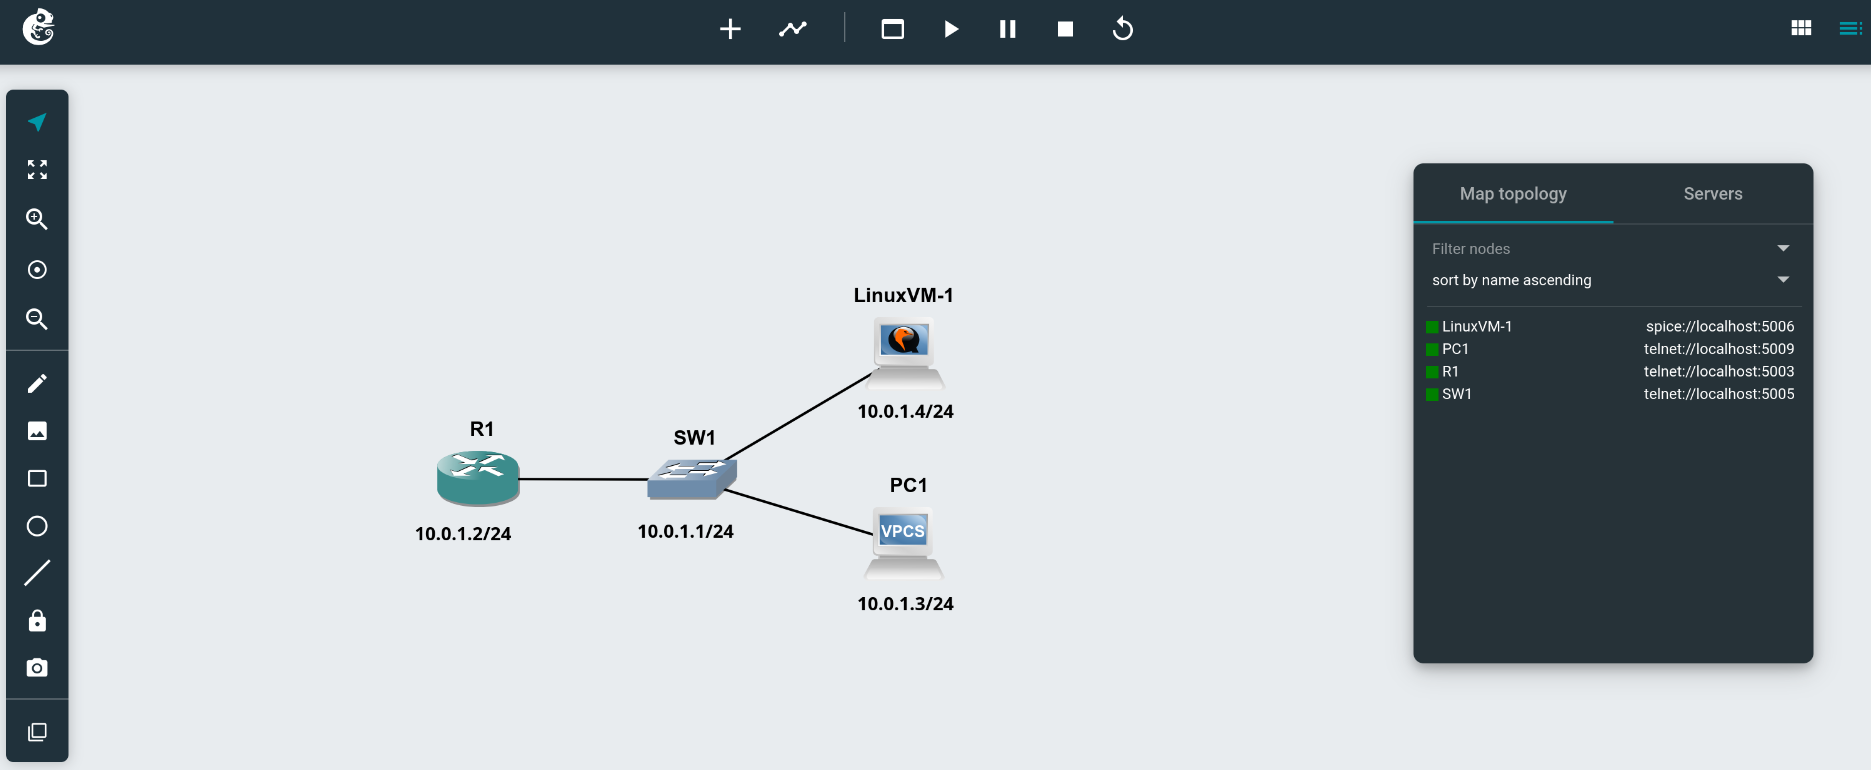
\includegraphics[width=.95\linewidth]
              {2Background/gns3-web.png}
          \caption{A simple network topology example in the GNS3 Web UI}
        \hfill
      \end{figure}


  \subsection{Proxmox VE} 
    \ac{pve} is an open-source platform designed for enterprise-level virtualization \cite{proxmox2025}. It is based on the Debian
    distribution of Linux and provides a web-based interface for managing virtual machines and containers. It is widely used
    in data centers and cloud environments, as it provides a scalable and reliable solution for virtualization.

    \ac{pve} bundles several core services that can be interacted with via shell commands, a web interface or by using
    the\ac{pve}\ac{rest}\ac{api}.
    These allow the user to interact with every service provided by\ac{pve}, in a plethora of ways, depending on the user's
    needs, skills and preferences. The web interface is the most user-friendly way to interact with the platform, as it
    provides a graphical interface for managing the cluster. The shell commands provide a more direct way to interact with the
    platform, allowing for more complex operations to be performed and opening the doors to scripting and automation. Finally,
    the\ac{pve}\ac{rest}\ac{api} allows for programmatic and remote interaction with the platform, enabling users to create custom
    applications that can interact with the platform.

    \subsubsection{Virtualization Technologies}
      \ac{pve} supports the the deployment and management of two distinct types of virtualization, namely,\ac{kvm} and\ac{lxc}.

      Users can interact with these virtualized environments via NoVNC, a simple web-based VNC client or\ac{spice} which is a more
      feature-rich protocol that provides better performance and more features than VNC.
      Both of these protocols support the use of a console-based interface, aswell as a full desktop graphical interface.

      \subsubsection{\ac{kvm}}
        \ac{kvm} is a virtualization solution provided by the Linux kernel. It leverages the hardware virtualization extensions 
        of modern processors to provide a full virtualization experience at near-native speeds. Supports a wide range of guest 
        operating systems making it a good choice for general purpose virtualization.

        In\ac{pve},\ac{kvm} is used as the core component for running virtual machines and is used alongside\ac{qemu}.

      \subsubsection{\ac{lxc}}
        Containerization is an operating system-level virtualization method that packages an application and its dependencies
        together into an isolated environment. Contrary to traditional\ac{vm} solutions, containers dont emulate hardware or require a 
        guest operating system relying instead on the host's kernel. This approach leads to a faster and more lightweight 
        virtualization solution, as they consume less memory and cpu resources.

        \ac{lxc} creates full system containers, capable of simulating a complete Linux distribution providing users with an 
        environment that behaves like a traditional\ac{vm} but with the speed and efficiency of a container.\ac{lxc} start 
        much faster than\ac{vm}s making them ideal for scenarios requiring rapid deployment and/or scaling.

        However, it's important to note that while containers offer a degree of isolation, they do not provide the same level of
        security as\ac{vm}s. This means that while they may not always be a suitable replacement for\ac{vm}s.

  \subsection{LDAP}

    \ac{ldap} is the foundation of user and device management in many institutions. Universities can rely on openLDAP and/or Microsoft's 
    Active Directory (its enterprise implementation) to handle student, faculty accounts and lab computer access, amongst other things.

    One of\ac{ldap}'s most popular implementations, OpenLDAP, had its initial release in 1998. The protocol's longevity stems from its 
    efficiency at handling large-scale authentication so much so that despite newer alternatives existing,\ac{ldap} remains entrenched 
    in academic environments due to its reliability and universal adoption. For our project,\ac{ldap} integration enables students 
    access to the system using their existing university credentials. 

    Two key factors make\ac{ldap} particularly valuable for this project: its standardized approach to user management 
    and pre-existing deployment in our target educational environments. Given the extensive use, it's desirable for our system to have the 
    capability to interact with LDAP in order to correctly authenticate users.

\section{Virtualized Lab Environments}
  The combined use of\ac{pve} as a virtualization platform and\ac{gns3} for network emulation presents a cost-effective solution for 
  scalable networking education. This approach offers significant benefits over physical lab infrastructures:

  \begin{itemize}
    \item \textbf{Resource Efficiency}: Single physical host can support multiple concurrent student environments
    \item \textbf{Operational Characteristics}:
    \begin{itemize}
        \item Accelerated environment provisioning through templates
        \item State preservation via\ac{pve}'s snapshot/restore functionality
        \item Support for diverse network operating systems through virtualization technologies
    \end{itemize}
  \end{itemize}

\section{Python Web Frameworks for API-Based Systems}

  \subsection{Python}
    Python is a high-level, interpreted programming language renowned for its readability and versatility. It supports 
    multiple programming paradigms, including procedural, object-oriented, and functional programming, making it suitable 
    for a wide array of applications.
    In the context of this project, Python serves as the primary programming language as its extensive standard library 
    and supportive community contribute to efficient development and maintenance of the project's codebase.

  \subsection{WSGI}
    The\ac{wsgi} is a pivotal standard for Python web application deployment, defining a consistent interface between web 
    servers and Python web applications/frameworks.

    Prior to\ac{wsgi}'s introduction\cite{pep333}, Python web frameworks were typically written against various server-specific APIs such as 
    CGI, FastCGI, or mod\_python. This diversity led to compatibility issues, limiting developers' choices of web servers and 
    frameworks, as not all frameworks supported all web servers and vice-versa. To address this fragmentation,\ac{wsgi} was 
    created as a standardized interface, promoting portability and flexibility in deploying Python web applications. 

    \ac{wsgi} serves as a bridge, enabling web servers to communicate with Python applications. It specifies a simple and universal 
    interface for web servers to forward requests to Python applications and for those applications to return responses. 
    This standardization allows developers to choose from a variety of web servers and Python frameworks without compatibility 
    concerns.

    Introduced in 2003 as PEP 333,\ac{wsgi} was later updated to PEP 3333 in 2010 to accommodate Python 3. These specifications 
    outline how web servers and Python applications should interact, ensuring a consistent and reliable deployment environment 
    across different platforms.

    The\ac{wsgi} standard consists of two main components:
    \begin{itemize}
      \item \textbf{Server/Gateway Side} - Responsible for receiving\ac{http} requests from clients and passing them to the 
      Python application. Then receives the response from the application and forwards it to the client. 
      \item \textbf{Application} - The Python application that processes requests and returns responses.
    \end{itemize}

    Additionally\ac{wsgi} has support for middleware components.\ac{wsgi} middleware is a Python callable that wraps another
    \ac{wsgi} application to observe or modify its behavior. Middleware can perform various functions, including request 
    preprocessing, response postprocessing, session management, and security checks. This modularity allows developers to 
    add functionality to their applications in a reusable and maintainable manner.

    The separation defined by\ac{wsgi} allows for flexibility and scalability in deploying Python web applications.

    Python\ac{wsgi} applications often use built-in servers, during development, provided by frameworks like Flask. 
    However, these servers typically aren't fully featured and aren't suitable for production environments. In production, WSGI 
    servers act as intermediaries between web servers (e.g., NGINX or Apache) and Python applications, handling incoming requests 
    and serving responses efficiently.

    \subsubsection{Flask}
      Flask is a web application micro framework written in Python, adhering to the\ac{wsgi} standard, designed to 
      facilitate the development of web applications by providing essential tools and features. Classified as a microframework, 
      Flask does not require particular tools or libraries, instead choosing to focus on simplicity and extensibility\cite{flask2025}.

      An example of how easy it is to develop a basic web application with flask is provided in the following small 
      piece of code.

      \begin{algorithm}
        \caption{Flask Hello World}\label{flask-hello-world}
        \begin{algorithmic}[1]
          \State \textbf{from} flask \textbf{import} Flask
          \State \textbf{app} = Flask(\_\_name\_\_)
          \State
          \State \textbf{@app.route('/')}
          \State \textbf{def} hello\_world():
          \State \hspace{1em} \textbf{return} 'Hello, World!'
          \State
          \State \textbf{if} \_\_name\_\_ == '\_\_main\_\_':
          \State \hspace{1em} app.run()
        \end{algorithmic}
      \end{algorithm}

  \subsection{ASGI}

    \ac{asgi} is an interface specification for Python web servers and applications. It is considered a spiritual successor to
    \ac{wsgi}, designed to provide a standard interface for asynchronous communication.\ac{asgi} was developed to address the 
    limitations of \ac{wsgi}, which was primarily designed for synchronous applications. Unlike\ac{wsgi},\ac{asgi} supports 
    handling multiple requests concurrently, making it suitable for modern web applications that require real-time features such 
    as WebSockets, long-lived connections, background tasks or the use of Python's async features.
    
    As development progressed, asynchronous task handling became a more central requirement, initially addressed by integrating 
    task queues. However, due to resource overhead and deployment complexity, they were phased out. This shift prompted an evaluation 
    of frameworks that offered native support for asynchronous operations.
    
    \subsubsection{FastAPI}
      
      FastAPI is a modern, high-performance web framework adopting the\ac{asgi} standard. It leverages open standards, such as 
      \ac{oas}, for defining path operations, parameters, and more, which in turn is based on the\ac{json} schema.
      FastAPI relies entirely on Python type declarations, making it more intuitive and lowering the barrier to entry to new 
      developers. This approach also simplifies the understanding and maintenance of the codebase.
      
      Built on top of Starlette, a lightweight\ac{asgi} framework, and Pydantic, a data validation library. FastAPI combines the 
      strengths of both to provide a powerful and flexible framework for building APIs with automatic data validation, 
      serialization and documentation generation, all of which significantly enhance developer productivity.
      
      Another key feature of FastAPI, being\ac{asgi}-compliant, is its built-in support for asynchronous programming, allowing 
      developers to write non-blocking code using Python's \textit{async}/\textit{await} keywords. This is particularly useful 
      for I/O-bound operations, such as database queries or network requests, as it allows the application to handle multiple 
      requests concurrently without blocking the application which is essential in projects such as this one where multiple 
      concurrent\ac{http} calls are made to interact with multiple devices and services concurrently, such as\ac{gns3} and\ac{pve}.
      
      Another powerful feature of FastAPI is its dependency injection system, that is very easy to use as it is automatically
      handled by the framework itselft. This allows for a clean and modular codebase, as dependencies can be easily injected into
      the various components of the application. This is especially useful in larger applications, where managing dependencies
      can become complex and cumbersome.
      
      A change from Flask to FastAPI laid the groundwork for more efficient handling of I/O-bound operations—such as network interactions 
      with\ac{pve} or\ac{gns3}, which will be of importance in future iterations of the project while also streamlining development thanks 
      to FastAPI's built-in request parsing, background task support, and integrated dependency injection system.

\section{Long running task processing approaches}

  \subsection{The need for asynchronous processing in API-heavy applications.}
    Modern\ac{api}-driven applications benefit tremendously from asynchronous programming paradigms to handle concurrent operations 
    efficiently. Traditional synchronous execution models, where each request blocks thread execution until completion, prove 
    inadequate for systems requiring high throughput and responsiveness. This limitation becomes particularly apparent in projects 
    like ours, which relies heavily on\ac{http} calls to various devices and services.

    The asynchronous model, implemented through Python's \texttt{async}/\texttt{await} syntax, offers several critical advantages:

    \begin{itemize}
        \item \textbf{Improved Resource Utilization}: A single thread can manage multiple concurrent I/O operations by yielding control during waiting periods
        \item \textbf{Enhanced Scalability}: Systems can handle higher concurrent user counts with the same hardware resources
        \item \textbf{Responsive Performance}: The application remains reactive even during long-running operations
    \end{itemize}

    Although Python has native asynchronous capabilities, libraries must be written with these in mind, meaning some may have limited 
    or even no support for these capabilities.
    
  \subsection{Asyncio}

    Asyncio is Python's built-in library for writing concurrent asynchronous code. It serves as the foundation for asynchronous operations 
    in many Python frameworks, enabling high-performance networking, web servers, database connections, distributed task queues, etc.. 

    Asynchronous I/O can be useful in cases of time-consuming operations, as while awaiting the finish of said tasks, it relinquishes control 
    so that other code can run in the meantime. This approach is particularly well-suited for I/O-bound operations—such as network 
    communication, file access, or database queries—where tasks would otherwise spend a significant amount of time waiting for external operations that 
    are outside of our control to complete. Rather than blocking the entire application during such waits, Asyncio allows other tasks to 
    execute in the meantime, leading to more efficient resource utilization and improved throughput.

    Overall, Asyncio provides the concurrency model that underpins efficient I/O performance. By embracing this model, 
    the project benefits from improved responsiveness, lower latency, and better scalability—especially under workloads that 
    involve heavy interaction with external services.

    Frameworks that leverage these capabilities natively, provide the foundation for building responsive, scalable\ac{api} 
    services.
    
  \subsection{Celery}
    Celery is an open source distributed task queue focused on real-time processing but also offers support for task scheduling.
    It is implemented in Python, but the underlying protocol can be implemented in any language. Celery requires a message broker 
    to function, such as Redis or RabbitMQ, which are responsible for queuing and distributing tasks from producers (clients) to 
    consumers (workers).

    When integrating Celery into their projects developers must mark functions they want to be processed as tasks with Celery provided 
    decorators (e.g. \texttt{@app.task}) which allows workers to then execute them asynchronously. The system shines in projects requiring 
    heavy computational or scheduled jobs, but brings with it non-negligible operational, developmental and resouce overhead, doubly so if 
    the project didn't already include the use of message brokers.

\section{System administration automation tools}

  Modern system administration increasingly relies on automation tools to manage complex infrastructure while maintaining reliability and 
  reproducibility. In our context, configuration management systems serve as the foundational layer for ensuring well-configured device states 
  across network environments.

  \subsection{Nornir}
  
    Nornir is an open-source automation framework written in Python, designed to provide a flexible and efficient 
    approach to network automation tasks\cite{nornir2025}. Unlike other automation tools that utilize customized 
    pseudo-languages, Nornir leverages pure Python code, offering developers the full power and versatility of the Python 
    ecosystem.

    Nornir supports multi-threaded task execution, allowing operations to run parallel across multiple devices.
    This capability enhances efficiency and reduces the time required enabling easy scaling to a large number of devices.

    The framework provides a robust inventory management system, enabling the organization of devices into groups and the 
    assignment of specific tasks to these groups. This structure facilitates targeted automation and simplifies complex 
    network operations.

    Finally, thanks to Nornir's architecture, it is highly extensible through its plugin system, allowing users to create 
    custom plugins for inventory management, task execution, and result processing. This modularity ensures that Nornir can 
    adapt to a wide range of network automation scenarios.

    Nornir makes it easy to write reusable tasks for configuration management and state validation which makes it 
    highly desirable in the context of this project. Its ability to handle concurrent operations will also ensure it can scale 
    alongside the rest of the project.

  \subsection{Ansible}

    Ansible is a widely adopted open-source automation platform that simplifies configuration management, application deployment, 
    and task automation through a declarative YAML-based approach. Unlike imperative scripting solutions, Ansible employs playbooks 
    to define system states, making automation accessible to both developers and operations teams while maintaining robust capabilities 
    for complex workflows.

    The platform operates on an agentless architecture, utilizing\ac{ssh} for connectivity, which eliminates the need for persistent software 
    on managed nodes. This design choice significantly reduces deployment overhead while maintaining secure communication through standard 
    protocols. Ansible's push-based execution model allows for immediate task execution across entire device inventories without requiring 
    pre-installed clients.

    Ansible remains a valuable tool in task automation and orchestration but, as was already discussed in\cite{santos2024} there are several 
    barriers to the adoption of Ansible in this project, mainly the difficulties encountered by utilizing the Telnet protocol for 
    communications with network devices that dont support the\ac{ssh} protocol .
% Chapter Template

% Main chapter title
%\chapter[toc version]{doc version}
\chapter{Related Work}

% Short version of the title for the header
%\chaptermark{version for header}

% Chapter Label
% For referencing this chapter elsewhere, use \ref{ChapterTemplate}
\label{Chapter3RelatedWork}

% Write text in here
% Use \subsection and \subsubsection to organize text

This chapter focuses on placing the current project within the context of existing solutions and related work. The primary 
goal of this project is to develop a system capable of automatically evaluating network topologies by validating device 
configurations and executing tests across a virtual network.

While automated assessment systems are well established in the field of programming education—receiving student-submitted 
code and running it against predefined test cases—equivalent systems for network exercises are far less common. Tools like 
Mooshak and similar platforms have proven effective for evaluating programming assignments and are widely adopted in academic 
settings.

At first glance, adapting these approaches to network topologies might seem straightforward. However, network evaluation 
introduces unique challenges such as the need for per-student virtual environments, real-time communication with multiple 
devices, and stateful, distributed configurations. This chapter explores existing tools like Mooshak and Packet Tracer, 
highlighting their capabilities, limitations, and how this project builds upon or diverges from them.

\section{Programming Evaluation Systems}
    While not directly related, they are the main inspiration for this project. Programming evaluation systems are widely
    deployed in universities and other educational institutions. These systems receive, as input, code from students and 
    subsequently run tests on it, outputting a score and even being configurable to provide students the first test case that 
    they failed in, guiding students to the solution without handing it out.

    The main differentiator between these systems and the one proposed in this project is the ability to solve a network 
    exercise using multiple configurations across multiple devices, while programming evaluation systems will expect
    the same output every time, given the same input.
    
    Another key difference is the fact that programming evaluation systems dont always provide a working environment for the 
    students to test their code, owing to the fact that students might prefer to user their own development environment for 
    initial development and testing. This project aims to provide a working environment for students, as setting up a 
    networking lab can be a daunting task for students, especially when they are just starting out. By providing a pre-configured
    environment, students can focus on learning the concepts and skills they need to succeed in their studies, rather than
    spending time troubleshooting their setup.

    \subsection{Mooshak and lessons learned}

        In our context, in the\ac{dcc}, Mooshak is commonly deployed to be used in the context of classes, exams and even 
        programming contests.

        Mooshak is a web-based system for managing programming contests and also to act as an automatic judge of programming 
        contests \cite{Leal2003567}. It supports a variety of programming languages like Java, C, etc. Under each contest students 
        will find one more problem definitions each containing varying sets of test cases in input-output pairs. After submiting 
        their solution, the system will compile and run the code against the test cases giving a score based on the the amount of 
        test cases passed.

        Mooshak provides a structured approach to test coding and problem solving skills. It begins by offering a problem statement 
        coupled with an optional image and an example test case, normally in the form of input and expected output.
        Users can submit their proposed solution by uploading a file with their code. The system then evaluates the provided solution 
        against multiple pre-defined test cases, validating the output against the know-good output, and giving feedback in the form of 
        a score based on the number of test cases passed. The system may also be configured to have time and/or memory constraints, 
        to ensure that temporal and spatial complexity are also taken into account.
    
        All of these, serve to provide a thorough evaluation of the student's solution, which can help guide a student to better
        their coding and problem solving skills.

        The system can also differentiate between differing types of errors, such as not giving the expected output, poorly 
        formatted output, failure to compile or even exceeding the time limits.
        Mooshak also includes some features designed to drive competition between students, like a real time leaderboard and
        the ability to have more than 100\% of the score for a given contest.

        The system however is not without its limitations as it uses plain text files for its test cases and validates the output 
        of student's code character by character, which can lead to false negatives if the output is not formatted exactly as
        expected.

\section{Cisco Packet Tracer}

    Cisco Packet Tracer is a network \textbf{simulation} tool developed by Cisco Systems, widely used in academic environments 
    to teach networking concepts and prepare students for certifications such as the Cisco Certified Network Associate (CCNA). 
    It offers a visual interface for building and simulating virtual network topologies using a variety of Cisco devices, 
    including routers, switches, and end devices.

    While Packet Tracer is highly accessible and effective for introducing networking fundamentals, it is a closed-source, 
    proprietary tool limited to simulating Cisco hardware and IOS features. Its functionality is optimized for teaching 
    purposes rather than for flexibility, extensibility, or integration into larger automated workflows.

    In contrast, this project aim to allow for a more realistic and extensible lab environment. The use of real operating 
    systems and support of a wide range of vendor platforms for routers and switches, aswell as Linux-based virtual machines 
    is highly desirable. This allows for a more realistic experience, as students will be able to work with the same tools and 
    operating systems that they will encounter in real-world scenarios.

    Therefore, while Cisco Packet Tracer remains a valuable educational tool, the needs of this project called for a more 
    flexible and open architecture.
% Chapter Template

% Main chapter title
%\chapter[toc version]{doc version}
\chapter{System Architecture \& Design}

% Short version of the title for the header
%\chaptermark{version for header}

% Chapter Label
% For referencing this chapter elsewhere, use \ref{ChapterTemplate}
\label{Chapter4SystemArchitectureDesign}

% Write text in here
% Use \subsection and \subsubsection to organize text

This chapter outlines the architecture of the proposed system, detailing the key components and how they interact to enable 
evaluation of student-submitted network exercises.

The system is designed to provide each student with a working environment where custom virtual network topologies can be 
deployed, configured, and tested. To achieve this, the platform integrates several technologies—such as\ac{gns3} for network 
emulation,\ac{pve} for virtualization, and Nornir for configuration testing—alongside an asynchronous web-based\ac{api} layer for 
user interaction and system communications.

This section provides a high-level overview of the system, the rationale behind its design choices, and the fundamental 
components that make up its architecture.

\section{Functional Use Cases}

\section{System Architecture Overview}
    The architecture is divided into several key components, each responsible for a specific aspect of the system's functionality. 
    The main components of the system architecture are as follows:

    \begin{itemize}
        \item \textbf{Web Application:} The web application serves as the main interface for users to interact with the system. It provides 
        endpoints for, amongst others, evaluation, creation  and viewing available exercises. The application is designed to be asynchronous 
        where possible, allowing for efficient handling of multiple requests simultaneously.
        
        \item \textbf{Proxmox VE:}\ac{pve} is responsible for creating and managing\ac{vm}s that host the network devices used in 
        the exercises. This component interacts with the web application and all communication is done asynchronously through 
        the\ac{pve}\ac{rest}\ac{api}, which allows for efficient communication, keeping the web application responsive, while also 
        keeping the components decoupled.
        
        \item \textbf{GNS3:}\ac{gns3} is used to emulate all the components of the virtual networks to be configured by students, 
        using various types of virtualization detailed earlier. Communication with\ac{gns3} is done through 
        the\ac{gns3}\ac{rest}\ac{api} by the web application during template\ac{vm} creation and validation

        \item \textbf{Nornir:} This automation framework is used for validating device configurations. It connects to the 
        virtualized devices, executes commands, and compares the output to expected results to determine correctness.
        Currently this component is integrated into the web application
    \end{itemize}

\section{Proxmox VE}

    \ac{pve} functions as the virtualization backbone of the system, enabling the creation and management of Linux-based\ac{vm}s 
    which in turn host services for use by students. Each\ac{vm} runs a lightweight Linux-based operating system with a 
    dedicated\ac{gns3} instance, providing a self-contained environment for deploying and configuring virtual networks 
    and their components.

    All\ac{pve}-related operations—such as cloning, starting, templating, and deletion—are fully automated and triggered by the 
    web application. Under normal operation ,after doing pre-required setup, no further manual intervention using the\ac{pve} web 
    UI or shell utilities is required; such intervention is only necessary when the system's error handling mechanisms detect failures 
    that cannot be automatically resolved. To securely execute these operations, the application authenticates to the\ac{pve}\ac{api} 
    using token-based authentication. The required credentials and configuration parameters are securely injected via environment variables\unsure{this may change}, 
    while the time limited token is stored in memory, ensuring that only authorized and properly configured processes can interact 
    with the\ac{pve} infrastructure.

    \subsection{Why Proxmox VE?}

        \ac{pve} was chosen for several compelling reasons that make it ideal for it to be choosen as our virtualization platform. First, 
        it's completely free to use for all core functionality, with no hidden costs or licensing traps. Unlike proprietary solutions that 
        charge per CPU core or socket,\ac{pve} lets us scale up our infrastructure without worrying about surprise licensing fees.

        The platform's support for both containers and\ac{vm}s within a single management interface gives us tremendous flexibility. We 
        can run lightweight\ac{lxc} for applications that dont require a full\ac{vm} while using full\ac{vm}s where required seamlessly. 
        This hybrid approach would not be as straightforward with other solutions, like VMware ESXi.

        We also value storage system's flexibility with LVM-thin provisioning allows efficient snapshotting of student environments while 
        maintaining good performance.

        Looking ahead,\ac{pve}'s built-in support for emerging technologies like software-defined networking and its robust role-based 
        access control system means our project still has room to grow into\ac{pve}. The active open-source development community ensures 
        continuous improvements without vendor lock-in.

    \subsection{Proxmox VE Limitations}

        During development, we encountered several challenges when interfacing programmatically with\ac{pve}. One of th most significant 
        issues stemmed from the platform's limited visibility into non-instantaneous operations - particularly for tasks like\ac{vm} cloning, 
        where the system did not provide task ids in the\ac{http} responses. This forced us to implement custom polling mechanisms to reliably 
        determine operation completion states where possible.

        A more critical limitation emerged in\ac{pve}ac{rest}ac{api}'s resilience characteristics. During stress testing, we discovered that 
        even moderate request volumes done using a single machine running sequential code could overwhelm the single-node cluster's management 
        daemon, triggering frequent\ac{http} 500 errors. These reliability constraints necessitated the development of protective measures 
        including exponential backoff retry logic and strict client-side concurrent request limiting to maintain system stability.

    \subsection{Proxmox VE Firewall}

        \ac{pve} comes bundled with a iptables-based firewall implementation that can be enabled and configured at different levels.

        The Proxmox host-level firewall provides essential features for securing student work environments, during examination 
        periods, preventing student machines and the virtualized network equipments in them from communicating with outside networks.

        This is done by adding firewall rules at the host level, meaning to each relevant student\ac{vm}, that disable communications
        in both directions, with the exception of the machine that is responsible for configuration validation.

        By default this behavior is not active and must be enabled on an as-needed basis, typically when a controlled assessment 
        environment is required for more rigorous situations such as examinations.

        In future iterations it may also be valuable to develop this further and making this feature less rigid as it may be interesting 
        to have exercises that communicate with devices on the internet.
    
    \subsection{Exploration of containers as a full substitute for VMs}

        During development, we attempted to minimize\ac{vm} usage where possible to accommodate as much scaling potencial as possible. 
        The introduction of the\ac{gns3} web interface allowed the machines hosting\ac{gns3} instances to operate in a headless manner, 
        removing the need for direct student interaction with the host machine. This eliminated desktop environment requirements and 
        significantly reduced memory overhead, improving scalability.

        We further explored replacing\ac{vm}s entirely with containers, which promised additional resource savings. However, this approach 
        proved unworkable due to fundamental technical constraints. Effective emulation requires\ac{kvm} acceleration, which presents 
        two problematic scenarios in containerized environments: either running unprivileged containers without\ac{kvm} access (resulting 
        in unacceptable performance degradation) or configuring privileged containers or containers with\ac{kvm} passthrough (introducing 
        serious security vulnerabilities).

        Given that software emulation without\ac{kvm} acceleration delivers poor performance for interactive use, we abandoned containerization 
        as a complete\ac{vm} replacement. The\ac{vm}-based architecture remains necessary to maintain both performance through hardware 
        acceleration and proper isolation between student environments.

        \subsubsection{VM Lifecycle}

            The lifecycle of a\ac{vm} begins when a new exercise is created by a priviledged user through the web application. 
            Upon exercise creation, the platform automatically clones a pre-configured base template\ac{vm} stored in\ac{pve}. This new instance 
            undergoes a configuration process where the provided\ac{gns3} project file is imported and a series of user-defined commands are executed 
            across the provided network topology. Once the setup is finalized, the configured\ac{vm} is converted into a new template\ac{vm} that 
            is tailored to that exercise.

            When students are enrolled in an exercise, the system generates individual work environments, by creating linked clones from these 
            exercise-specific templates. Each student receives their own isolated\ac{vm} instance that precisely mirrors the original template's 
            configuration. This cloning approach ensures both consistency across student environments and rapid provisioning, as linked clones 
            avoid the overhead of full disk copies while maintaining the template's baseline configuration. The use of linked clones significantly 
            reduces both storage requirements and deployment time compared to traditional full cloning methods.
        
\section{GNS3}

    \ac{gns3} serves as the core network virtualization component in our system, providing the capability to emulate various network devices 
    and topologies. The platform was selected for several key advantages: its remote web-based interaction, the intuitive drag-and-drop interface 
    simplifies usage, and its broad device support accommodates both terminal-based and GUI network equipment and full computers. Additionally, 
    \ac{gns3}'s\ac{api} allows for programmatic interaction, which proves essential for automation within our environment.

    Currently, the system requires manual preparation of the base \ac{gns3} template\ac{vm}. During initial setup, an administrator must first create 
    and configure a new\ac{vm}, then proceed to install and set up the\ac{gns3} environment. The final preparation step involves importing all 
    necessary device images, including routers, switches, and other equipment that will be available for student exercises.

    This base template then serves as the source for all subsequent student instances through\ac{pve}'s cloning functionality. While this 
    manual setup process adds initial configuration overhead, it ensures complete control over the base environment and allows for careful 
    curation of the included device images.

    The system achieves scalability through multiple \ac{vm} instances running in \ac{pve}, each hosting an independent \ac{gns3} environment. 
    This architecture enables concurrent usage by multiple students on a single physical host. For future expansion, the design supports 
    horizontal scaling by adding additional nodes to the \ac{pve} cluster, allowing the platform to accommodate growing numbers of users 
    without requiring complete architectural changes.

    \begin{figure}
        \centering
          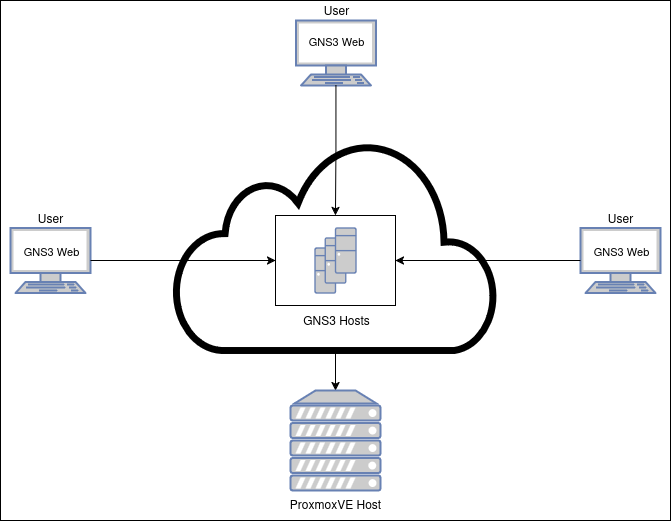
\includegraphics[width=.95\linewidth]
            {4SystemArchitectureDesign/user-gns3-proxmox-diagram.png}
        \caption{A diagram showcasing how users interact with the system's resources on a high level}
      \hfill
    \end{figure}

\section{High-level architecture}

    \subsection{Available Hardware}

        The current deployment hosts all internal system components (those shown in the architecture diagram excluding the external LDAP instance) 
        on a single physical server with the following specifications.

        \begin{table}[h]
            \centering
            \caption{System Hardware Specifications}
            \begin{tabular}{|l|l|}
                \hline
                \textbf{Component} & \textbf{Specification} \\ \hline
                Processor & Intel Core i7-9700K \\ \hline
                Memory & 32GB DDR4 @ 2666MHz \\ \hline
                Storage & 1TB Samsung 970 EVO Plus NVMe SSD \\ \hline
                Graphics & NVIDIA GTX 1650 \\ \hline
            \end{tabular}
        \end{table}

        This machine's specifications, while capable enough for development purposes, create inherent memory constraints. With 32GB of available RAM, 
        practical\ac{vm} allocation becomes the primary bottleneck. For instance, when deploying\ac{gns3} instances each configured with 4GB of memory, 
        the system can maintain only seven active\ac{vm}s simultaneously. This limitation accounts for the\ac{pve} hypervisor's own memory overhead 
        before inducing SWAP file usage, which would degrade performance.

    \subsection{User Interface}
        The system employs a dual-interface web architecture accessible through standard browsers. For administrative functions and exercise management, 
        users interact with Jinja2-rendered HTML pages delivered by the web application. These templates handle all developed features, like user 
        authentication,\ac{vm} interaction etc.

        When working on networking exercises, users can transition to the \ac{gns3}-web interface by clicking a button. This dedicated environment 
        provides direct access to the user's virtual network devices, as required by each exercise scenario. This integration ensures users experience 
        a cohesive workflow from exercise selection to practical implementation without needing multiple authentication steps or application switches.

    \subsection{Web Application}

        The web application serves as the primary interface through which users interact with the system. It is built using the FastAPI 
        framework, following a migration from an earlier prototype developed using Flask, and follows an asynchronous-first, modular 
        architecture that provides scalable interactions with other system components.

        The application exposes a\ac{rest}\ac{api} that supports endpoints for user authentication, exercise creation, virtual 
        machine management, and configuration validation. It acts as the coordinator for the entire system, triggering operations 
        in\ac{pve},\ac{gns3}, and Nornir based on user actions.

        Wherever possible, asynchronous I/O is employed to prevent blocking during operations such as\ac{api} calls to\ac{pve}.
        Multiprocessing is also utilized to handle configuration validation. This keeps the system responsive and performant, 
        especially when handling multiple simultaneous requests from different users.

        Internally, the application is designed to be stateless and maintain minimal runtime state.  Most essential information—such 
        as user accounts, defined exercises, and student-to-VM mappings—is persisted in a relational database rather than stored in 
        memory. Configuration values such as API tokens, base URLs, and database credentials are injected via environment variables 
        to decouple deployment-specific settings from the application code. This design improves reliability, supports concurrent 
        usage, and enables horizontal scalability if deployed across multiple instances. 

        To ensure maintainability and modularity, interactions with external services like\ac{pve} and\ac{gns3} are isolated in 
        dedicated modules. These serve as abstraction layers between the application logic and third-party\ac{api}s, exposing clean, 
        reusable interfaces while hiding low-level implementation details. For example,\ac{pve}-related operations such as\ac{vm} 
        creation and deletion are handled in a separate module (e.g services/proxmox.py), as are all\ac{gns3}-related tasks. This 
        separation of concerns improves the structure of the codebase and simplifies future maintainability by being more readable.

        To help with development and testing, the application automatically generates OpenAPI-compliant documentation, allowing 
        developers to explore and interact with available endpoints. This self-documenting behavior streamlines integration 
        testing and encourages a more agile development process.

        Finally, to safeguard user data and infrastructure control points, the application enforces secure authentication mechanisms 
        using\ac{jwt} ensuring that only authorized users can trigger actions on shared resources.

    \begin{figure}
        \centering
            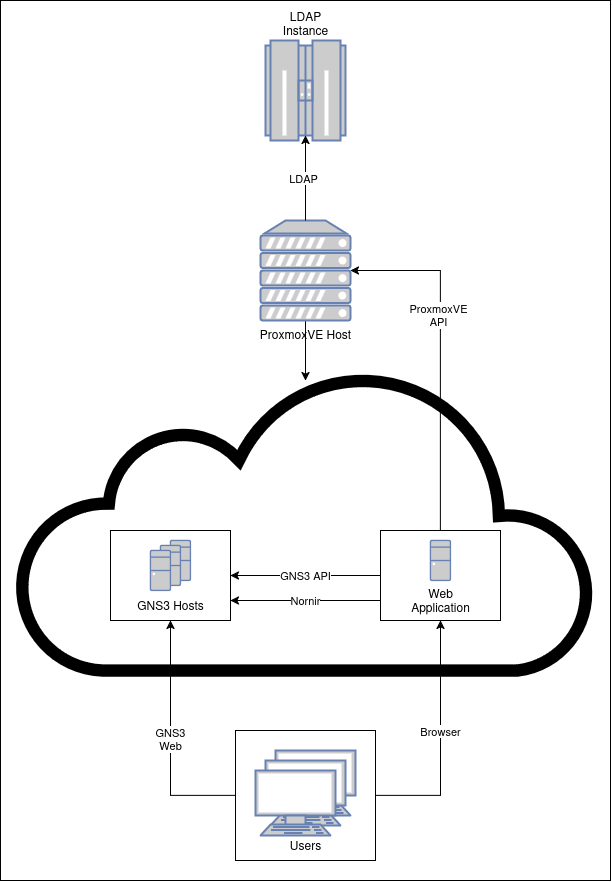
\includegraphics[width=.95\linewidth]
                {4SystemArchitectureDesign/system-diagram.png}
            \caption{A diagram showcasing a high level overview of the system's main components}
        \hfill
    \end{figure}

    \subsection{Virtualization Components}

        The system employs a hybrid virtualization approach using\ac{pve} as the foundational platform. The usage of containers was 
        explored but it was found unsuitable for our main use case of virtualization,\ac{gns3} instances. However there remains one valid 
        usage for containers for the project, which is hosting the web application. However this component may also be optionally hosted in 
        a separate physical machine.

        For network emulation, the system utilizes full\ac{kvm}-based virtual machines, each hosting a\ac{gns3} instance. These\ac{vm}s 
        provide the necessary hardware virtualization support for nested device emulation, particularly crucial for fast virtualization. 
        Finally, by the use of linked clones and storage-efficient backing filesystems, in this case LVM-thin, allows the system to rapidly 
        provision\ac{vm}s while minimizing storage usage.
    
    \subsection{Evluation component}

        The system employs a modular evaluation framework built on Nornir to validate configurations across virtualized network devices. 
        At its core, this component utilizes specialized Python classes called "modules" that encapsulate platform-specific validation logic. 
        Each module is responsible for three key functions: identifying the target device's platform (such as Cisco IOS, Linux, or VPCS), 
        executing the appropriate validation commands for that platform, and interpreting the command output using regular expressions to d
        etermine configuration correctness.

        The architecture follows an object-oriented design pattern with a base \texttt{CommandModule} class that handles common functionality. 
        This parent class manages the Nornir inventory initialization and provides essential methods like platform detection and command execution. 
        The actual validation logic is implemented in child classes that inherit from \texttt{CommandModule}, with each subclass specializing in 
        a particular type of network test. For example, the included \texttt{PingModule} implements platform-specific variants of the ping command 
        and corresponding response interpretation methods. This design promotes code reuse while allowing easy extension for new test types, as 
        developers can create additional modules by simply extending the base class and implementing the required platform-specific methods.
        
        Configuration validation occurs through a multi-stage process. When a test is initiated, the system first identifies the target device's 
        platform through Nornir's inventory system. It then dispatches the appropriate platform-specific command variant, such as the Cisco IOS-style 
        ping command for routers versus the Linux \texttt{ping -c} syntax for Linux hosts. The module captures and sanitizes the raw command output, 
        removing terminal control sequences and other artifacts before applying regular expressions to assess the results. For connectivity tests like 
        ping, the interpretation logic calculates success rates against a configurable tolerance threshold defined in the system constants.
        
        The evaluation framework supports several advanced features to enhance reliability and debugging. Command timeouts are managed to prevent 
        hanging operations, with a default window that can be tuned as needed. Future extensions could incorporate snapshot functionality, allowing 
        the system to capture and compare device states at different points during an exercise, though this capability is not currently implemented 
        in the base version. The modular architecture ensures such enhancements can be added without disrupting existing validation workflows.

    \subsection{Storage component}
        
        The system has two main components regarding storage, one for the database needs of the web application and one for the disks of the \ac{vm}s.

        \subsubsection{Virtual machine storage}

            \ac{lvmt} is an efficient solution for creating and managing virtual machines (VMs) by optimizing storage usage and improving performance. Unlike 
            traditional\ac{lvm}, which pre-allocates disk space,\ac{lvmt} allows dynamic allocation, meaning storage is consumed only as the\ac{vm} writes 
            data—ideal for environments like ours where multiple \ac{vm}s share the same storage pool. When combined with\ac{cow} snapshots, \ac{lvmt} enables 
            rapid\ac{vm} cloning and backup operations. For instance, a base\ac{vm} image can serve as a template, and new\ac{vm}s are created as linked 
            clones that initially share all data blocks with the original. Only when a\ac{vm} modifies its disk does\ac{lvmt} allocate new blocks, 
            significantly reducing storage overhead. This approach not only saves disk space but also speeds up\ac{vm} deployment, making it a great choice for 
            our project. Additionally, since snapshots are space-efficient, in the future, we can maintain multiple VM checkpoints without worrying about excessive 
            storage consumption—as long as the thin pool is monitored to avoid overprovisioning. Overall,\ac{lvmt} provides a scalable, high-performance storage 
            layer for virtualization with minimal waste.

        \subsubsection{Web application database}

            The SQLite database serves as the central repository for all application data, leveraging SQLModel as an ORM layer that combines Pydantic 
            validation with SQLAlchemy's database capabilities. This hybrid approach provides both runtime type safety and efficient database operations, 
            while Alembic handles schema migrations to accommodate evolving data requirements.

            The database schema organizes information across several interrelated models. User management builds upon a base \texttt{CustomBase} class 
            that automatically tracks creation timestamps, with the \texttt{User} model storing authentication credentials, administrative privileges, 
            and relationships to both submissions and virtual machine instances. The \texttt{Exercise} model captures lab configuration details, including 
            \ac{json}-serialized validation rules and device configurations stored as text fields due to SQLite's native type limitations.\ac{vm} 
            provisioning is managed through the \texttt{TemplateVm} and \texttt{WorkVm} hierarchy, where template instances maintain the base\ac{gns3} 
            project configurations and spawned work environments link back to both users and exercises. The \texttt{Submission} model completes the 
            core data structure by tracking student attempts, scores, and evaluation outputs while maintaining referential integrity through SQLModel 
            relationships.

\section{FastAPI Adoption: Overcoming Flask's Shortcomings}

    \subsection{Initial setup: Flask}

        Initially, Flask served as the framework for the web application, providing the necessary infrastructure to handle \ac{http} 
        requests, render templates, and manage application routing. Its flexibility and minimalistic approach allow for the 
        integration of various extensions and libraries as needed, ensuring the application remains lightweight yet functional. 
        Flask's comprehensive documentation and supportive community further enhance its suitability by the creation and support
        of community-driven extensions speeding up development and reducing the need to reinvent the wheel.

        However, as development progressed, the need for better I/O performance became increasingly apparent. Early on, it was 
        clear that leveraging Python's native \textttt{asyncio} would benefit the project—but a significant portion of the existing codebase, 
        including Flask itself, relied on non-async-compatible libraries. This limitation stemmed from Flask's foundation on\ac{wsgi}, a 
        synchronous standard developed long before Python's asyncio was introduced.\ac{wsgi} operates strictly in a blocking request-response 
        model, requiring each request to complete fully before processing the next. While traditional workarounds like multi-threading 
        or multi-processing can mitigate this, they introduce complexity and are better suited for CPU-bound tasks than I/O-bound workloads.

        To address these constraints, several approaches were considered:

        \begin{itemize}
            \item \textbf{Gevent/Eventlet:} These libraries use monkey-patching to emulate asynchronous behavior in synchronous code. However, 
            they are not true asyncio and can lead to unpredictable behavior. Given the project's early stage, this option was deemed too risky

            \item \textbf{Flask + Celery:} Offloading long-running tasks to Celery workers helps avoid blocking but introduces operational overhead, 
            requiring additional infrastructure like Redis or RabbitMQ for message brokering

            \item \textbf{Quart (ASGI Flask):} A Flask-compatible\ac{asgi} reimplementation with native async/await support. However, Quart lacks 
            Flask's mature ecosystem and still relies partially on monkey-patching, raising concerns about long-term stability

            \item \textbf{FastAPI (Full ASGI migration):} Built on\ac{asgi}, FastAPI was designed with async-first principles, enabling efficient handling 
            of thousands of concurrent connections. Its native async/await support and modern tooling offer a cleaner solution without the need 
            for workarounds, at the expense of having to reimplement some features already implemented in Flask
        \end{itemize}

        While Flask remained suitable for early development, emerging requirements—particularly those involving asynchronous 
        communication for more scalable I/O operations—eventually led to a need to explore architectural shifts, due to 
        Flask's limited async support and\ac{wsgi} heritage. 
    
    \subsection{Second setup: Flask + Celery}

        As the limitations of Flask's synchronous\ac{wsgi} model became more apparent, we explored Celery as a potential solution for handling 
        asynchronous tasks. Celery, a distributed task queue system, allows offloading blocking I/O to separate worker processes. 
        Celery operates by decoupling task execution from the main application flow. When a time-consuming operation is required, Flask 
        dispatches it to a Celery worker via a message broker (typically Redis or RabbitMQ). The worker processes the task asynchronously, 
        while Flask remains free to handle incoming requests. While this approach mitigated some of Flask's blocking I/O issues, it 
        introduced new challenges in complexity and system overhead.

        The Celery architecture operates through worker processes that listen to the message broker for tasks. These workers run as 
        independent processes, executing tasks marked with Celery's \texttt{@app.task} decorator. The system's concurrent processing 
        capability comes from multiple workers operating in parallel, each handling different tasks from the queue. Tasks are Python 
        functions that are decorated with provided Celery decorators such as \texttt{@app.task}, causing them to be registered as 
        Celery tasks within the Celery application. This design is particularly valuable for operations like batch processing or 
        scheduled jobs that would otherwise block Flask's synchronous request handling.

        \begin{algorithm}
            \caption{Calling a Celery Task and Getting the Result}\label{celery-call-result}
            \begin{algorithmic}[1]
            \State \textbf{from} celery \textbf{import} Celery
            \State
            \State \textbf{app} = Celery('tasks', broker='redis://localhost:6379/0', backend='redis://localhost:6379/0')
            \State
            \State \textbf{@app.task}
            \State \textbf{def} hello():
            \State \hspace{1em} \textbf{return} 'hello world'
            \State
            \State \textbf{result} = hello.delay()
            \State \textbf{print}(result.get())
            \end{algorithmic}
        \end{algorithm}

        To execute a task, a Celery task function must be called using the \textit{delay()} method, which will return a result object. 
        This result object can be used to check the status of the task and to retrieve the result once it is available.

        Celery supports horizontal scaling by design, allowing multiple worker pools to run on separate physical or virtual machines. 
        This makes it especially effective for handling growing workloads—for example, processing email newsletters for an expanding 
        user base.

        Celery's advanced features, including task retries, chaining, and prioritization, while powerful, further increased the 
        system's complexity. We found ourselves managing not just our application logic, but also the reliability of the message broker, 
        persistence of results, and supervision of worker processes. This architectural overhead seemed increasingly disproportionate to 
        our actual needs as the project evolved.

        Furthermore, Celery clients and workers introduce a non-negligible overhead in terms of CPU and memory usage, even when 
        idle, as they must maintain persistent connections to the broker and periodically perform health checks or heartbeats. 
        This can be a concern in resource-constrained environments or during development.This overhead became especially evident 
        during early integration tests.

        As the project evolved and tests were performed, it became increasingly clear that Celery's benefits lend themselves better 
        to CPU-bound workloads, as opposed to our I/O-bound ones, and they did not outweigh its resource and architectural costs for 
        the current use case. This realization prompted an exploration of more lightweight asynchronous alternatives, eventually 
        culminating in an investigation into \ac{asgi}-compliant frameworks with native async capabilities and simpler concurrency 
        management.

    \subsection{Third setup: Quart, an ASGI-compliant Flask reimplementation}

        Quart emerged as a promising candidate during our exploration of async solutions, offering a unique combination of 
        Flask syntax with\ac{ASGI} compliance. As a near-drop-in replacement for Flask, Quart theoretically allowed for 
        an easy migration while providing all the benefits of native async/await support. The framework's design promised 
        seamless execution of asynchronous code alongside familiar Flask patterns, making it particularly attractive for 
        existing Flask projects that would benefit from asynchronous capabilities.

        However, practical evaluation revealed significant limitations in Quart's ecosystem maturity. While the core framework 
        maintained good compatibility with code orignally written for Flask and critical extensions we relied on - including 
        authentication, database integration, among others - either lacked Quart equivalents or had poorly maintained 
        implementations. We discovered many Quart-specific packages were either abandoned, documented only through sparse 
        READMEs, or failed to match their Flask counterparts in functionality. For instance, the Flask-Login equivalent for Quart 
        was one such unmaintained extension that would require some reimplementation. This gap would require us to reimplement 
        substantial portions of our web application instead of using existing, known-good solutions.

        While Quart offers the possibility to use monkey patching on Flask extensions, deeper evaluation revealed this 
        compatibility came with significant trade-offs. This approach could make some Flask extensions work in the 
        async environment, we found this to be an unstable foundation for long-term maintenance. Notably, recent Quart 
        releases have started to moved away from this approach  - the framework now treats these compatibility layers 
        as optional extras rather than core features, signaling a deliberate shift in architectural direction.

        Additionally, Quart's smaller community and limited production adoption made it difficult to assess long-term viability, 
        raising concerns about framework maintenance and the availability of future support.

        Ultimately, while Quart's technical merits as an\ac{asgi} Flask alternative were sound, the ecosystem risks and migration 
        costs outweighed its benefits for our project. The framework's current state appears best suited for teams that 
        can commit to Quart's entire stack, rather than as a migration path for existing Flask applications with extension 
        dependencies. This realization steered us toward more mature\ac{asgi} alternatives, despite requiring some 
        reimplementation, that could provide robust async support without sacrificing ecosystem stability.

    \subsection{Final Decision: FastAPI Migration}

        After thorough evaluation of the previous options, we ultimately selected FastAPI as our framework of choice. 
        The decision was driven by FastAPI's native \ac{ASGI} support, which provides built-in asynchronous capabilities 
        without requiring additional infrastructure components. Unlike our Flask + Celery implementation that demanded 
        separate worker processes and message brokers, FastAPI achieves comparable performance under high concurrency through 
        asyncio-compatible architecture, which enables concurrent non-blocking I/O, while significantly reducing system 
        complexity and operational overhead. The framework's performance characteristics proved particularly advantageous 
        for our I/O-bound operations, matching Celery's throughput in load testing but having a simpler application 
        architecture.

        The transition to FastAPI brought multiple technical benefits beyond just asynchronous capabilities. The framework's 
        integrated OpenAPI documentation generation and Pydantic-based data validation significantly improved our development 
        workflow and API reliability. While the migration required adapting our route handlers and dependency management 
        patterns, this investment was offset by FastAPI's excellent documentation and growing ecosystem. FastAPI emerged as 
        the most balanced solution, combining mature production readiness with modern features and approachable syntax. 
        The framework's design addressed our immediate performance requirements but also established a solid foundation for 
        future enhancements.
% Chapter Template

% Main chapter title
%\chapter[toc version]{doc version}
\chapter{Implementation}

% Short version of the title for the header
%\chaptermark{version for header}

% Chapter Label
% For referencing this chapter elsewhere, use \ref{ChapterTemplate}
\label{Chapter5Implementation}

% Write text in here
% Use \subsection and \subsubsection to organize text


% Chapter Template

% Main chapter title
%\chapter[toc version]{doc version}
\chapter{Testing \& Evaluation}

% Short version of the title for the header
%\chaptermark{version for header}

% Chapter Label
% For referencing this chapter elsewhere, use \ref{ChapterTemplate}
\label{Chapter6TestingEvaluation}

In this chapter were will go over how we did performance and stress tests aswell as discuss the results seen.

\section{Performance Evaluation}

    To evaluate the impact of migrating from Flask (+ Celery) to FastAPI, we conducted a series of measurements 
    focusing on the following metrics:

    \begin{itemize}
        \item \textbf{Time to complete a given task.}
        \item \textbf{CPU resources consumption.}
    \end{itemize}

    Each test consisted of three sequential tasks:

    \begin{enumerate}
        \item \textbf{1st task: Template\ac{vm} creation:} A new\ac{vm} was cloned from a pre-configured template. Once 
        cloning was complete, the\ac{vm} was powered on, waited for to acquire a valid IP address, and had a 
        project imported into its\ac{gns3} instance. After the import was processed, the\ac{vm} was powered off 
        and converted into a template.

        \item \textbf{2nd task:\ac{vm} cloning:} Immediately after the template was ready, a predetermined number of clones 
        were created from it.

        \item \textbf{3rd task:\ac{vm} deletion:} Finally, the newly created\ac{vm}s and the template were deleted.
    \end{enumerate}

    To eliminate human error as much as possible, human intervention was only required to trigger the 1st and the 
    3rd tasks.

    Each batch test was performed for different quantities of\ac{vm} clones: 1, 10, 20, 100, and 200. The execution 
    times for each task were logged for analysis.

    \subsection{I/O Problems during Batch VM Operations}

        During stress tests of mass cloning and deletion of\ac{vm}s (200 at a time, dispatched to a single\ac{pve} 
        node), we observed rising task times, specifically for the mass cloning of new\ac{vm}s, as can be seen in 
        the following graph

        \begin{figure}[h]
        \centering
        \begin{tikzpicture}
            \begin{axis}[
            ybar,
            bar width=7pt,
            width=\textwidth,
            height=9cm,
            ylabel={Time (s)},
            xlabel={Batch Number},
            symbolic x coords={1,2,3,4,5},
            xtick=data,
            ymin=0,
            enlarge x limits=0.2,
            legend style={at={(0.5,-0.2)}, anchor=north,legend columns=3},
            ymajorgrids=true,
            bar shift auto
            ]

            % Template creation (no labels)
            \addplot+[ybar, fill=gray] coordinates {
            (1,34.379) (2,34.312) (3,34.422) (4,34.609) (5,34.571)
            };
            \addlegendentry{Template Creation}

            % VM cloning (with labels)
            \addplot+[
            ybar,
            fill=black,
            nodes near coords,
            every node near coord/.append style={
                font=\small,
                anchor=south,
                rotate=90,
                yshift=2pt
            }
            ] coordinates {
            (1,86.187) (2,97.805) (3,110.508) (4,125.758) (5,152.186)
            };
            \addlegendentry{VM Cloning}

            % VM deleting (no labels)
            \addplot+[ybar, fill=gray!60] coordinates {
            (1,4.612) (2,4.942) (3,5.377) (4,0.0) (5,7.090)
            };
            \addlegendentry{VM Deleting}

            \end{axis}
        \end{tikzpicture}
        \caption{Grouped bar chart showing VM operation times. Cloning time is labeled to highlight the rising trend. Results
        from Flask running purely sequential code}
        \label{fig:vm_grouped_cloning_focus}
        \end{figure}

        It was also noted that there was an error during the 4th batch of tasks, specifically during the deleting task.

        After some investigation it was found that there were intermittent failures to remove\ac{vm} disks. These failures 
        were \emph{not} detectable via the standard\ac{http}\ac{api} responses and only appeared in the\ac{pve} server 
        logs. As orphaned disks accumulated, overall performance degraded significantly.

        \medskip
        \noindent\textbf{Observed Task History Outputs:}
        \begin{verbatim}
            --- 1st type of output (VM disks removed successfully) ---
            trying to acquire lock...
            OK
            Logical volume "vm-348786940-disk-0" successfully removed.
            TASK OK

            --- 2nd type of output (intermittent lock-timeout failures) ---
            trying to acquire lock...
            Could not remove disk 'local-lvm:vm-120993831-disk-0', check manually:
            can't lock file '/var/lock/pve-manager/pve-storage-local-lvm' - got timeout
            trying to acquire lock...
            OK
            Logical volume "vm-120993831-disk-0" successfully removed.
            TASK OK

            --- 3rd type of output (persistent failures) ---
            trying to acquire lock...
            Could not remove disk 'local-lvm:vm-363495383-disk-0', check manually:
            can't lock file '/var/lock/pve-manager/pve-storage-local-lvm' - got timeout
            trying to acquire lock...
            can't lock file '/var/lock/pve-manager/pve-storage-local-lvm' - got timeout
            TASK OK

            --- 4th and final type of output (storage config update errors) ---
            trying to acquire lock...
            Could not remove disk 'local-lvm:vm-5469324-disk-0', check manually:
            can't lock file '/var/lock/pve-manager/pve-storage-local-lvm' - got timeout
            trying to acquire lock...
            can't lock file '/var/lock/pve-manager/pve-storage-local-lvm' - got timeout
            trying to acquire cfs lock 'file-user_cfg' ...
            TASK OK
        \end{verbatim}

        This suggests\ac{pve}'s locking mechanism can't keep pace with the fast paced mass amount of delete requests. 
        The lock is used to ensure that two tasks dont modify the\ac{lvm}'s metadata simulatenously. Since there should be 
        some background tasks that are piling up, the system cant keep pace and eventually starts using retries to keep 
        up but even this is insuficient and starts failing more and more towards the end as it becomes fully congested. 
        At the end the system starts becoming overwhelmed and also begins having trouble updating its internal storage 
        config file.  

        This, combined with other factors were the main reason that led us to implement a hard limit on the amount of concurrent 
        requests that can be made from the web application to\ac{pve}\ac{api}. Still, while this significantly reduces the chances 
        of this problem reocurring, it does not fully remedy the problem and additional future work should look into solving this 
        matter completely.

        After performing a cleanup of the orphaned disks we can see that performance was improved from even the 1st baseline test

        \begin{figure}[h]
        \centering
        \begin{tikzpicture}
            \begin{axis}[
                ybar,
                bar width=20pt,
                width=\textwidth,
                height=9cm,
                ylabel={Time (s)},
                xlabel={Scenario},
                symbolic x coords={After Cleanup, Baseline, Worst Run},
                xtick=data,
                ymin=0,
                enlarge x limits=0.3,
                legend style={at={(0.5,-0.2)}, anchor=north, legend columns=1},
                ymajorgrids=true
            ]

            % VM cloning bars without labels
            \addplot+[
                ybar,
                fill=black
            ] coordinates {
                (After Cleanup,70.954)
                (Baseline,86.187)
                (Worst Run,152.186)
            };
              
            \addlegendentry{VM Cloning}

            \end{axis}
        \end{tikzpicture}
        \caption{Bar chart showing VM cloning times after cleanup, at baseline, and in the worst case scenario.}
        \label{fig:vm_grouped_cloning_focus}
        \end{figure}




% Write text in here
% Use \subsection and \subsubsection to organize text


% Chapter Template

% Main chapter title
%\chapter[toc version]{doc version}
\chapter{Conclusion \& Future Work}

% Short version of the title for the header
%\chaptermark{version for header}

% Chapter Label
% For referencing this chapter elsewhere, use \ref{ChapterTemplate}
\label{Chapter7ConclusionFutureWork}

% Write text in here
% Use \subsection and \subsubsection to organize text



% Add others as needed


%-------------------------------------------------------------------------
%	BIBLIOGRAPHY
%-------------------------------------------------------------------------
\addvspacetoc{0.5cm}
\addtotoc{Bibliography}

%\fancyhead[LO]{\textsc{Bibliography}}

 % The references are stored in the file "Bibliography.bib"
\bibliography{Bibliography}

%-------------------------------------------------------------------------
%	THESIS CONTENT - APPENDICES
%-------------------------------------------------------------------------

\appendix % Cue to tell LaTeX that the following 'chapters' are Appendices

%%% -----------  ADD APPENDIX HERE ------------------ %%%

% Appendix Template

\chapter*{Appendix Title Here} % Main appendix title

\label{AppendixX} % Change X to a consecutive letter; for referencing this appendix elsewhere, use \ref{AppendixX}

Write your Appendix content here.
%\input{Appendices/AppendixB}
%\input{Appendices/AppendixC}

\backmatter


\end{document}
